\documentclass[12pt,a4paper]{book}
\usepackage[utf8]{inputenc}
\usepackage[romanian]{babel}
\usepackage{amsmath}
\usepackage{amsfonts}
\usepackage{amssymb}
\usepackage{hyperref}
\author{Mihai Cornel}
\title{Python Tkinter}

\usepackage{graphicx} 
\usepackage{listings}
\usepackage{xcolor}

\begin{document}
\section{Python Tkiner}
	Tkinter este un modul Python pentru crearea interfețelor grafice(GUI) și este inclus în toate distribuțiile standard Python. Acest modul oferă o interfață pentru setul de instrumente Tk și funcționează pe modelul orientat obiect. Setul de instrumente Tk este o colecție multiplatformă de elemente de control grafic, cunoscute sub numele de widget-uri, pentru construirea interfețelor grafice.
Pentru verificarea versiunii Tcl/Tk în terminal introduceți:
\begin{verbatim}
$ tclsh
% info patchlevel
	8.6.10
\end{verbatim}
Pentru a verifica instalarea corectă a modulului Tkinter în terminal introduceți comanda:
\begin{verbatim}
$ python3 -m tkinter
\end{verbatim}
Această comanda deschide următoarea fereastră:

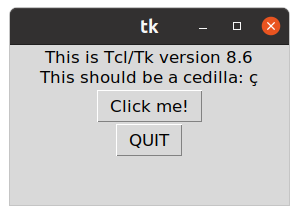
\includegraphics[width=\linewidth]{/home/mhcrnl/Desktop/Blog/img02.png}

Acest modul oferă utilizatorilor Python o modalitate simplă de a crea elemente grafice folosind widgeturile găsite în setul de instrumente Tk.  Widget-urile Tk pot fi folosite pentru a construi butoane, meniuri, câmpuri de date etc. într-o aplicație Python.  Odată create, aceste elemente grafice pot fi asociate sau pot interacționa cu caracteristici, funcționalitați, metode, date sau chiar alte widgeturi. 
De exemplu, un widget de buton poate accepta clicuri de mouse și poate fi, de asemenea, programat pentru a efectua un fel de acțiune, cum ar fi ieșirea din aplicație.
	
	Aceasta este un program Python cu Tkinter și rezultatul după rularea programului:
\lstinputlisting[language=Python]{main01.py}
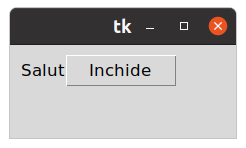
\includegraphics[width=\linewidth]{img01.png}

\section{Python tkinter.ttk}
Vechile widget-uri clasice Tkinter le-a introdus în 1991.
Cele mai noi widget-uri tematice ttk au fost adăugate în 2007 cu Tk 8.5.  Cele mai noi widget-uri tematice ttk înlocuiesc multe (dar nu toate) widget-uri clasice.
Există diferite moduri de a importa modulul ttk. Dacă preferați ca toate widget-urile și alte caracteristici ale Tkinter și ttk să fie în spațiul dvs. de nume global, utilizați această formă de import:
\begin{verbatim}
  from tkinter import *
  from ttk import *
\end{verbatim}
	Este important să faceți aceste două importuri în această ordine, astfel încât toate tipurile de widget-uri de la ttk să înlocuiască widget-urile echivalente de la Tkinter.  De exemplu, toate widgeturile Button vor proveni de la ttk și nu de la Tkinter.
    În aplicații mai complexe, unde utilizați mai multe module importate, poate îmbunătăți foarte mult lizibilitatea codului dvs. dacă practicați o igienă sigură a spațiului de nume: importați toate modulele dvs. folosind sintaxa „import modulename”.  Acest lucru necesită doar un pic mai mult de tastare, dar are marele avantaj că puteți privi o referință la ceva și puteți spune de unde a venit.
\begin{verbatim}
   import ttk
\end{verbatim}
 	După acest import, ttk.Label este constructorul widge-tului Label, ttk.Button este un Button și așa mai departe.
Dacă trebuie să faceți referire la articole din modulul Tkinter, acesta este disponibil sub numele de ttk.Tkinter.  De exemplu, codul de ancorare pentru „nord-est” este ttk.Tkinter.NE.
În schimb, puteți importa Tkinter separat în acest fel:
\begin{verbatim}
   import Tkinter as tk
\end{verbatim}
     După această formă de import, codul pentru „nord-est” este tk.NE.
     
\subsection{Button}
Widget-ul Button reprezintă un element care poate fi apăsat (clik) în aplicații.  De obicei, utilizați un text sau o imagine pentru a afișa acțiunea care va fi efectuată atunci când faceți clic.

	Butoanele pot afișa text într-un singur font.  Cu toate acestea, textul poate cuprinde mai multe linii.  În plus, puteți face unul dintre caracterele subliniate pentru a marca o comandă rapidă de la tastatură.

Pentru a invoca automat o funcție sau o metodă a unei clase atunci când se face clic pe buton, atribuiți opțiunea de comandă funcției sau metodei.  Aceasta se numește legarea comenzii în Tkinter.

Pentru a crea un buton, utilizați constructorul ttk.Button după cum urmează:
\begin{verbatim}
  buton = ttk.Button(container, **option)
\end{verbatim}
Un buton are multe opțiuni.  Cu toate acestea, cele tipice sunt acestea:
\begin{verbatim}
  buton = ttk.Button(container, text, command)
\end{verbatim}
În această sintaxă:

     * container este componenta părinte pe care plasați butonul.
     
     * text este eticheta butonului.
     
     * command specifică o funcție de apel invers care va fi apelată automat atunci când butonul a fost apăsat.\ldots
\subsubsection{Buton simplu}
\lstinputlisting{main03.py}
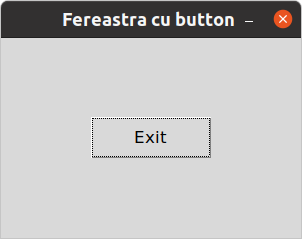
\includegraphics[width=\linewidth]{img03.png}

\subsection{Checkbox}
O casetă de selectare este un widget care vă permite să bifați și debifați.

 O casetă de selectare poate conține o valoare și poate invoca un apel invers atunci când este bifată sau debifată.

 De obicei, utilizați o casetă de selectare atunci când doriți să cereți utilizatorilor să aleagă între două valori.

 Pentru a crea o casetă de selectare, utilizați constructorul ttk.Checkbutton:
 
\begin{verbatim}
 checkbox_var = tk.StringVar()

 def check_changed():
    #...

 checkbox = ttk.Checkbutton(container,
                text='<checkbox label>',
                command=check_changed,
                variable=checkbox_var,
                onvalue='<value_when_checked>',
                offvalue='<value_when_unchecked>')
\end{verbatim}
Următorul program ilustrează modul de utilizare a unui widget casetă de selectare.  După ce bifați sau debifați caseta de selectare, o casetă de mesaj va afișa valoarea activată și valoarea oprită în consecință:
\lstinputlisting{main04.py}
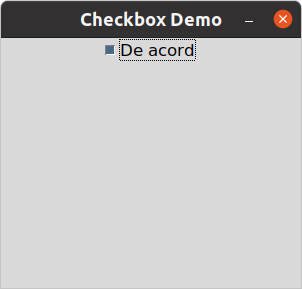
\includegraphics[width=\linewidth, scale=0.25]{img04.png}

\subsection{Entry}
Widget-ul Entry vă permite să introduceți o linie de text. În Tkinter, pentru a crea o casetă text se utilizează widget-ul Entry.
\begin{verbatim}
    textbox = ttk.Entry(container, **options)
\end{verbatim}
\begin{itemize}
\item container este fereastra părinte, unde este plasat widget-ul
\item options sunt unul sau mai multe argumente cheie pentru a configura widget-ul
\end{itemize}
Pentru a obține textul curent al unui widget Entry se utilizează metoda get():
\begin{verbatim}
    textbox.get()
\end{verbatim}
De obicei, se asociază valoarea curentă a casetei de text cu un obiect StringVar astfel:
\begin{verbatim}
    # Instanta clasei StringVar care va contine textul
    text = tk.StringVar()
    # Atribuirea variabilei text widget-ului Entry
    textbox = ttk.Entry(root, textvariable=text)
\end{verbatim}
În acest caz, putem utiliza apelarea metodei get() obiectului StringVar() pentru a obține valoarea curentă a widget-ului Entry:
\begin{verbatim}
    text.get()
\end{verbatim}



\subsection{Frame}

\subsection{Label}

\subsection{LabelFrame}

\subsection{MenuButton}

\subsection{PanedWindow}

\subsection{Radiobutton}

\subsection{Checkbox}

\subsection{Scale}

\subsection{Scrollbar}

\subsection{Spinbox}

\subsection{Combobox}

\subsection{Notebook}

\subsection{Progressbar}

\subsection{Separator}

\subsection{Sizegrip}

\subsection{Treeview}

Tkinter ttk \url{https://www.pythontutorial.net/tkinter/tkinter-ttk/}
 
\begin{verbatim}
  print(“Hello, World!”) 
\end{verbatim} 

@online{example,
    title = {Example.com},
    url   = {http://www.example.com},
}

   

	



  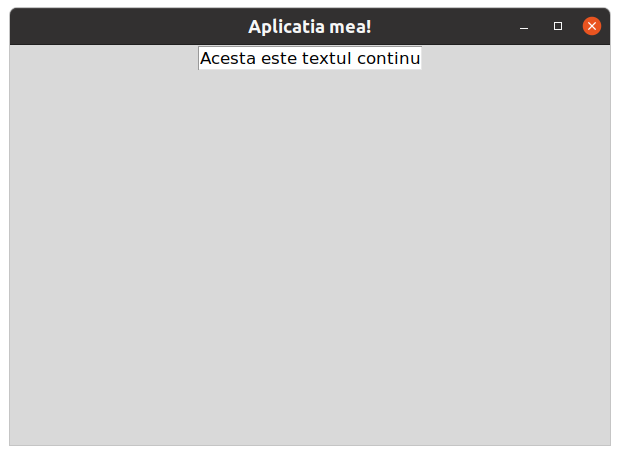
\includegraphics[width=\linewidth, scale=0.25]{/home/mhcrnl/Desktop/Blog/oct2021/pyart04/img01.png}
  
 






\end{document}
